%% -*- fill-column: 72; eval: (auto-fill-mode -1); eval: (visual-fill-column-mode 1); eval: (visual-line-mode 1); eval: (adaptive-wrap-prefix-mode 1) -*-
\documentclass[10pt, a4paper]{article}
\usepackage{amsmath}
\usepackage{amsthm}
\usepackage{amssymb}
\usepackage[margin=0.51in]{geometry}
\usepackage{parskip}
\usepackage{tabularx}
\usepackage{array}
\usepackage{changepage}
\usepackage[mathscr]{euscript}
\usepackage{hyperref}
\usepackage{graphicx}

\newcommand{\defn}[1]{\textbf{\textsf{#1}}}
\newcommand{\set}[1]{\mathbold{#1}}
\newcommand{\imag}{\mathrm{i}}
\def\R{\mathbb{R}}
\def\C{\mathbb{C}}
\def\F{\mathbb{F}}
\def\setsep{\mid}
\def\vspan{\text{span}}
\def\enumfix{\mbox{ } \vspace*{-1.2\baselineskip}}
\def\deg{\mathop{\text{deg}}}
\def\dim{\mathop{\text{dim}}}
\def\f{f}
\def\finv{f^{-1}}

\newtheoremstyle{break}% name
  {}%          Space above, empty = `usual value'
  {8pt}%       Space below
  {\upshape}%  Body font
  {}%          Indent amount (empty = no indent, \parindent = para indent)
  {\bfseries}% Thm head font
  {.}%         Punctuation after thm head
  {\newline}%  Space after thm head: \newline = linebreak
  {}%          Thm head spec

\theoremstyle{break}
\newtheorem{innerresult}{Result}

\newenvironment{result}[1]
  {\renewcommand\theinnerresult{#1}\innerresult}
  {\endinnerresult}

\title{Vector Space Bijection}
\date{9 December 2023}
\author{}

\renewcommand{\arraystretch}{1.2}
\setlength{\tabcolsep}{3pt}

\newenvironment{forceindent}{\begin{adjustwidth}{16pt}{}}{\end{adjustwidth}}

%%%%%%%%%%%%%%%%%%%%%%%%%%%%%%%%%%%%%%%%%%%%%%%%%%%%%%%%

\begin{document}

\maketitle

%%%%%%%%%%%%%%%%%%%%%%%%%%%%%%%%%%%%%%%%%%%%%%%%%%%%%%%%

\section*{Bijections of Vectors Spaces}

\begin{result}{1.0}[Bijections of Vectors Spaces are Vector Spaces]
Let $\F$ be a field, $V$ a vector space over $\F$ and $X$ a set such that
$$
\f : V \to X
$$
is a bijection (one-to-one and onto). Then we can understand $X$ as a vector space over $\F$ by setting
\begin{align*}
+      & : X \times X \to X \\
\times & : \F \times X \to X
\end{align*}
such that
\begin{align*}
v + w & \mapsto \f( \finv(v) + \finv(w)) \\
a v   & \mapsto \f( a \finv (v))
\end{align*}
\end{result}
\begin{proof}
We need to demonstrate that the set $X$ satisfies the definition for a vector space (Definition 1.20 in Axler 4th edition): commutativity, associativity, additive identity, additive inverse, multiplicative identity and the distributive property.

In the steps below, where it says ``by bijectivity of $\f$'' we're making use of the fact that $\finv$ is the inverse of $\f$, so $\finv \circ \f = 1$ (the identity map), hence we can add or remove cases of $\f(\finv(x))$ at will.

\defn{Commutativity}

Let $u, v \in X$. Then
\begin{align*}
u + v & = \f( \finv (u) + \finv(v)) && \text{by definition of $+$}, \\
      & = \f( \finv (v) + \finv(u)) && \text{by commutativity in $V$}, \\
      & = v + u.
\end{align*}

\defn{Associativity}

Let $u, v, w \in X$. Then
\begin{align*}
(u + v) + w & = \f( \finv( \f( \finv(u) + \finv(v))) + \finv(w)) && \text{by definition of $+$}, \\
            & = \f(( \finv(u) + \finv(v)) + \finv(w)) && \text{by bijectivity of $\f$}, \\
            & = \f( \finv(u) + ( \finv(v) + \finv(w))) && \text{by associativity in $V$}, \\
            & = \f( \finv(u) + \finv( \f( \finv(v) + \finv(w)))) && \text{by bijectivity of $\f$}, \\
            & = u + (v + w) && \text{by definition of $+$}.
\end{align*}

Let $a, b \in \F$ and $v \in V$. Then
\begin{align*}
(ab)v & = \f((ab) \finv(v)) && \text{by definition of $\times$}, \\
      & = \f(a (b \finv(v))) && \text{by associativity in $V$}, \\
      & = \f(a \finv( \f( b \finv(v)))) && \text{by bijectivity of $\f$}, \\
      & = \f(a \finv(bv)) && \text{by definition of $\times$}, \\
      & = a(bv) && \text{by definition of $\times$}.
\end{align*}

\defn{Additive identity}

Since $V$ is a vector space we know that there is an additive identity $0_V \in V$. Set $0_X = \finv(0_V)$. We claim that $0_X$ is the additive identity in $X$:

\begin{align*}
v + 0_X & = \f( \finv(v) + \finv(0_X)) && \text{by definition of $+$}, \\
        & = \f( \finv(v) + 0_V) && \text{by definition of $0_X$}, \\
        & = \f( \finv(v) && \text{since $0_V$ is the additive identity in $V$}, \\
        & = v && \text{by bijectivity of $\f$}.
\end{align*}

\defn{Additive inverse}

For $v \in X$ we know that $\finv(v) \in V$. Since $V$ is a vector space we know that $\finv(v)$ has an additive inverse $-\finv(v) \in V$. Set $w = \f( -\finv(v)) \in X$. Then
\begin{align*}
v + w & = \f( \finv(v) + \finv( \f( -\finv(v))) && \text{by definition of $+$}, \\
      & = \f( \finv(v) - \finv(v)) && \text{by bijectivity of $\f$}, \\
      & = \f(0_V) && \text{by additiive inverse in $V$}, \\
      & = 0_X && \text{by definition of $0_X$}.
\end{align*}

\defn{Multiplicative identity}

Let $v \in X$. Then
\begin{align*}
1 v & = \f(1 \times \finv(v)) && \text{by definition of $\times$}, \\
    & = \f( \finv(v)) && \text{by multiplicative identity in $V$}, \\
    & = v && \text{by bijectivity of $\f$}.
\end{align*}

\defn{Distributive property}

Let $a \in \F$ and $u, v \in X$. Then
\begin{align*}
a(u + v) & = \f(a \finv(u + v)) && \text{by definition of $\times$}, \\
         & = \f(\ \finv( \f( \finv(u) + \finv(v)))) && \text{by definition of $+$}, \\
         & = \f(a (\finv(u) + \finv(v))) && \text{by bijectivity of $\f$}, \\
         & = \f(a \finv(u) + a \finv(v)) && \text{by distributivity in $V$}, \\
         & = \f( \finv( \f( a \finv(u))) + \finv( \f( a \finv(v)))) && \text{by bijectivity of $\f$}, \\
         & = \f( \finv(au) + \finv(av)) && \text{by definition of $\times$}, \\
         & = au + av && \text{by definition of $+$}.
\end{align*}

Let $a, b \in \F$ and $v \in X$. Then
\begin{align*}
(a + b) v & = \f((a + b) \finv(v)) && \text{by definition of $\times$}, \\
          & = \f( a \finv(v) + b \finv(v)) && \text{by distributivity in $V$}, \\
          & = \f( \finv( \f(a \finv(v))) + \finv( \f( b \finv(v)))) && \text{by bijectivity of $\f$}, \\
          & = \f( \finv(av) + \finv(bv)) && \text{by definition of $\times$}, \\
          & = av + bv && \text{by definition of $+$}.
\end{align*}

Since all of the properties are met it follows that $X$ is a vector space when $+$ and $\times$ are as defined.
\end{proof}

\section*{Unit Sphere as a Vector Space}

The above tells us that if we can find a bijection from a vector space to any other set, then we can also represent the set as a vector space. Let's define $S^2$ to be the unit sphere with centre $(0, 0, 0)$ like this:
$$
S^2 = \{ (x, y, z) \in \R^3 \setsep x^2 + y^2 + z^2 = 1 \}.
$$

The sets $S^2$ and $\R^2$ have the same cardinality so we can find a bijection between them which we {\it could\/} use to impose a vector space structure on $S^2$.

However, as already noted during the session there is no bijection between $\R^2$ and a sphere that preserves continuity. A bijection that is continuous and with a continuous inverse is called a \defn{homeomorphism}\footnote[1]{\url{https://en.wikipedia.org/w/index.php?title=Homeomorphism&oldid=1185280979}} and is what we'd ideally want for the vector space on the sphere to be useful.

On the other hand we {\it can\/} find a homeomorphsim between $\R^2$ and a sphere with a single point (usually one of the poles) removed. One example is the stereographic projection. Embed $\R^2$ into $\R^3$ as the plane
$$
\R^2 = \{ (x, y, z) \in \R^3 \setsep z = 0 \}.
$$

Then $S^2 \setminus \{ (0, 0, 1) \}$ is the sphere with the north pole removed. Let $\mathscr{M} = S^2 \setminus \{ (0, 0, 1) \}$.

We can find a homeomorphism between $\R^2$ and $\mathscr{M}$ as follows. For any point $(x, y, 0) \in \R^2$ draw a line from the north pole of the sphere through the point $(x, y, 0)$ on the plane. The line will intersect the sphere at exactly one point (other than the north pole). The point at which it crosses is the point on the sphere that $(x, y, 0)$ maps to.

\begin{figure}[h!]
\centering
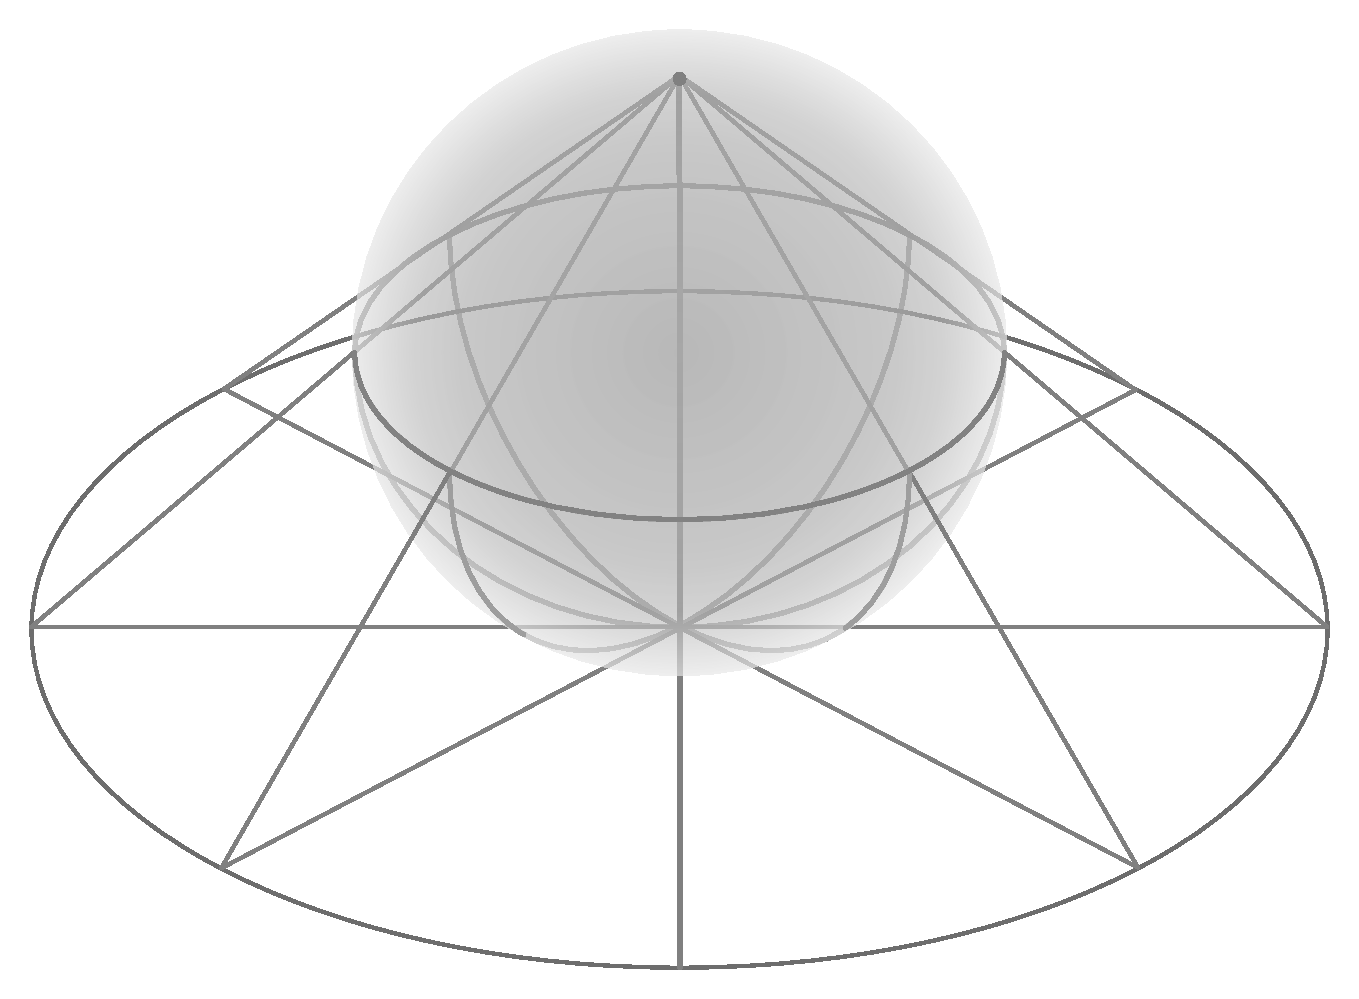
\includegraphics[width=0.5\linewidth]{./figures/stereoproj.pdf}
\caption[Stereographic projection]{Stereographic projection between the plane $\R^2$ and the north-poleless-sphere $\mathscr{M}$. Image from Wikipedia, Mark Howison and CheChe, CC BY-SA 4.0 Deed\footnotemark[2].}
\label{fig:stereoproj}
\end{figure}

\footnotetext[2]{\url{https://commons.wikimedia.org/wiki/File:Stereographic_projection_in_3D.svg}}

Using this approach every point on the $\R^2$ plane maps uniquely to a point on $\mathscr{M}$ and any point on $\mathscr{M}$ maps uniquely to a point on $\R^2$.

We can define the mapping $\f : \R^2 \to \mathscr{M}$ and its inverse $\finv : \mathscr{M} \to \R^2$ as follows.
\begin{align*}
\f (x, y) & \mapsto \left( \frac{2x}{1 + x^2 + y^2}, \frac{2y}{1 + x^2 + y^2}, \frac{-1 + x^2 + y^2}{1 + x^2 + y^2} \right), \\
\finv (x, y, z) & \mapsto \left( \frac{x}{1 - z}, \frac{y}{1 - z} \right).
\end{align*}

For the derivation see Wikipedia\footnote[3]{\url{https://en.wikipedia.org/w/index.php?title=Stereographic_projection&oldid=1183460764}}.

Since $\f$ is a bijection we can consider $\mathscr{M}$, the unit sphere minus a pole, as being a vector space by defining vector addition and scalar multiplication as earlier. So let $(x_1, y_1, z_1), (x_2, y_2, z_2) \in \mathscr{M} \subset \R^3$ and $a \in \R$ then
\begin{align*}
(x_1, y_1, z_1) + (x_2, y_2, z_2) & \mapsto \f( \finv((x_1, y_1, z_1)) + \finv((x_2, y_2, z_2))) \\
a (x_1, y_1, z_1) & \mapsto \f( a \finv ((x_1, y_1, z_1))).
\end{align*}

If we want (I'm not sure we do) we can expand these out by working through all of the functions and inverse functions. The formula for addition of vectors in $X$ then becomes the following.

\begin{align*}
(x_1, y_1, z_1) + (x_2, y_2, z_2) & = \left( \frac{2(x_1 (1 - z_2) + x_2 (1 - z_1)(1 - z_1)^2(1 - z_2)^2}{(1 - z_1)^2 (1 - z_2)^2 + (x_1(1 - z_2) + x_2(1 - z_1)^2 + (y_1(1 - z_2) = y_2(1 - z_1))^2)}, \right. \\
& \qquad \qquad \left. \frac{2(y_1 (1 - z_2) + y_2 (1 - z_1)(1 - z_1)^2(1 - z_2)^2}{(1 - z_1)^2 (1 - z_2)^2 + (x_1(1 - z_2) + x_2(1 - z_1)^2 + (y_1(1 - z_2) = y_2(1 - z_1))^2)}, \right. \\
& \qquad \qquad \qquad \qquad \left. \frac{(x_1(1 - z_2) + x_2(1 - z_1))^2 + (y_1(1 - z_2) + y_2(1 - z_1))^2 - (1 - z_1)^2(1 - z_2)^2}{(x_1(1 - z_2) + x_2(1 - z_1))^2 + (y_1(1 - z_2) + y_2(1 - z_1))^2 + (1 - z_1)^2(1 - z_2)^2} \right). \\
\intertext{While the formula for scalar multiplication is the following.}
a \times (x, y, z) & = \left( \frac{2ax(1 - z)}{(1 - z)^2 + a^2 x^2 + a^2 y^2}, \frac{2ay(1 - z)}{(1 - z)^2 + a^2 x^2 + a^2 y^2}, \frac{a^2 x^2 + a^2 y^2 - (1 - z)^2}{a^2 x^2 + a^2 y^2 + (1 - z)^2} \right)
\end{align*}

In these two equations addition, multiplication and division are all operations on the underlying field $\R$. These remind me of the formulas for addition and scalar multiplication in $\C$ from Axler (Definition 1.1): although they don't look much like addition and multiplication they still satisfy all of properties from Definition 1.20.

Since $\{ (1, 0), (0, 1) \}$ is a basis for $\R^2$ we can find a basis for $\mathscr{M}$ as:
\begin{align*}
\{ \f((1, 0)), \f((0, 1)) \} & = \left\{ \left( \frac{2 \times 1}{1 + 1^2 + 0^2}, \frac{2 \times 0}{1 + 1^2 + 0^2}, \frac{-1 + 1^2 + 0^2}{1 + 1^2 + 0^2} \right), \left( \frac{2 \times 0}{1 + 0^2 + 1^2}, \frac{2 \times 1}{1 + 0^2 + 1^2}, \frac{-1 + 0^2 + 1^2}{1 + 0^2 + 1^2} \right) \right\} \\
                             & = \left\{ \left( \frac{2}{2}, \frac{0}{2}, \frac{0}{2} \right), \left( \frac{0}{2}, \frac{2}{2}, \frac{0}{2} \right) \right\} \\
                             & = \left\{ \left( 1, 0, 0 \right), \left( 0, 1, 0 \right) \right\} . \\
\intertext{The additive identity element in $\mathscr{M}$ is:}
\f((0, 0))                   & = \left( \frac{2 \times 0}{1 + 0^2 + 0^2}, \frac{2 \times 0}{1 + 0^2 + 0^2}, \frac{-1 + 0^2 + 0^2}{1 + 0^2 + 0^2} \right) \\
                             & = (0, 0, -1).
\end{align*}

It's worth noting that all three of these are (thankfully) points on the unit sphere.



\end{document}
